\documentclass[handout]{beamer}

\usepackage{fontspec} 
\useoutertheme{lsp}

\usepackage{lsptitle}

\def\two@digits#1{\ifnum#1<10 0\fi\number#1}
\def\mytoday{\two@digits{\number\day}.\two@digits{\number\month}.\number\year}


\usepackage{xspace,multicol}
\newcommand{\latex}{\LaTeX\xspace}
\usepackage{tikz}


\newcounter{lastpagemainpart}
\footnotesep0pt
\renewcommand{\footnoterule}{}
\usefootnotetemplate{
  \noindent
  \insertfootnotemark\insertfootnotetext}

\let\beamerfn=\footnote
\renewcommand{\footnote}[1]{%
\let\oldfnsize=\footnotesize%
\let\footnotesize=\tiny%
\beamerfn<\thebeamerpauses->{#1}%
\let\footnotesize=\oldfnsize}


\date{\today}

\usepackage{eurosym}  
 
\renewcommand{\centerline}[1]{\hfill#1\hfill\hfill\mbox{}}


\title{\mbox{Open Monograph Press}}
% \institute{FU Berlin}
\author[Nordhoff]{Sebastian Nordhoff}



\begin{document}
\lspbeamertitle

\section{Was ist OMP}

\frame{ 
\frametitle{Was ist OMP}
\begin{itemize}
 \item  Plattform zur Veröffentlichung von Monographien
 \item  angelehnt an OJS (Zeitschriften)
 \item  webbasiert  
 \item  Open Source
\end{itemize}
}

\frame{ 
\frametitle{Was ist OMP}
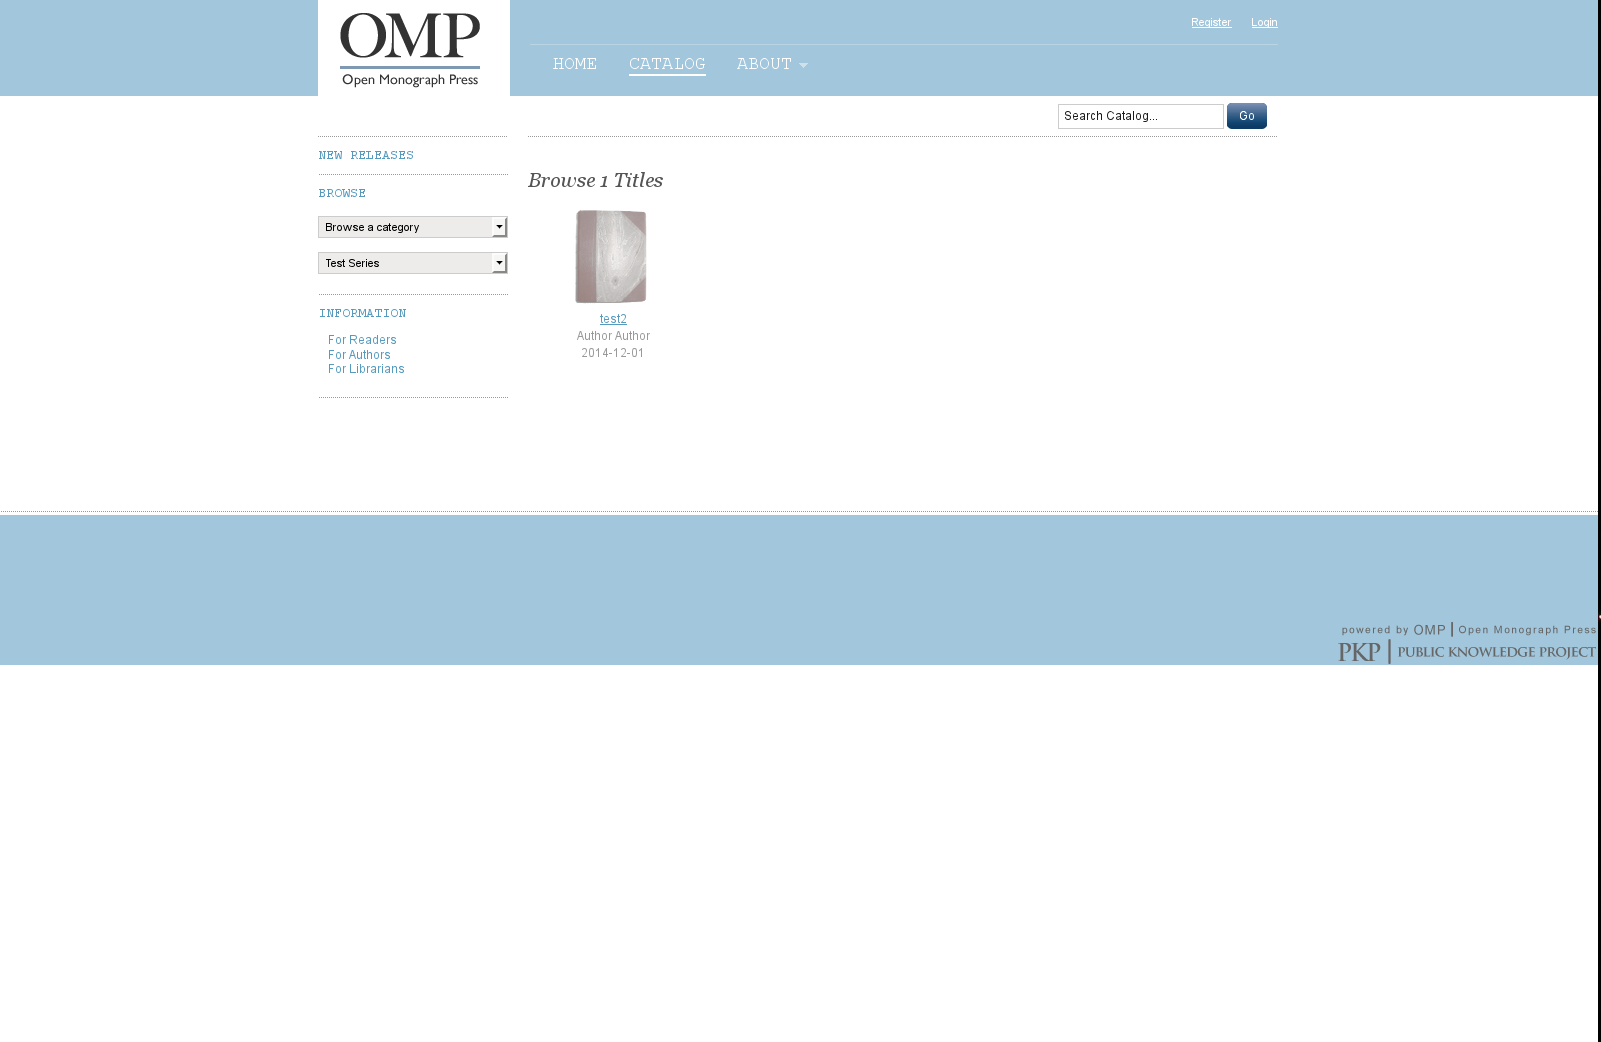
\includegraphics[\width=\textwidth]{./pics/ompdev.png}
}

\frame{ 
\frametitle{Was ist OMP}
\begin{itemize}
 \item von PKP in Kanada entwickelt
 \item weltweit eingesetzt
 \item PHP+js+CSS/LESS 
 \item kann auch für Closed Access eingesetzt werden, mit Vertriebsregionen
\end{itemize}
}

\section{Was leistet OMP}

\frame{ 
\frametitle{Was leistet OMP}
\begin{itemize}
 \item   Dokumentenverwaltung
 \item   Begleitung durch den Publikationsprozess in 5 Phasen
 \item   Benutzerverwaltung mit verschiedenen Rollen
 \item   Pluginsystem
\end{itemize}
}

\frame{ 
\frametitle{Was leistet OMP}
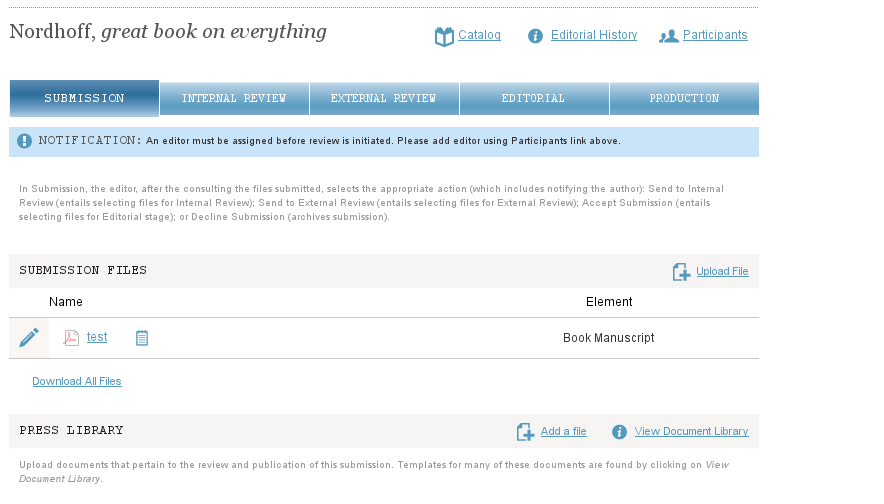
\includegraphics[\width=\textwidth]{./pics/omporigsubmission.png}
}

\frame{ 
\frametitle{Was leistet OMP}
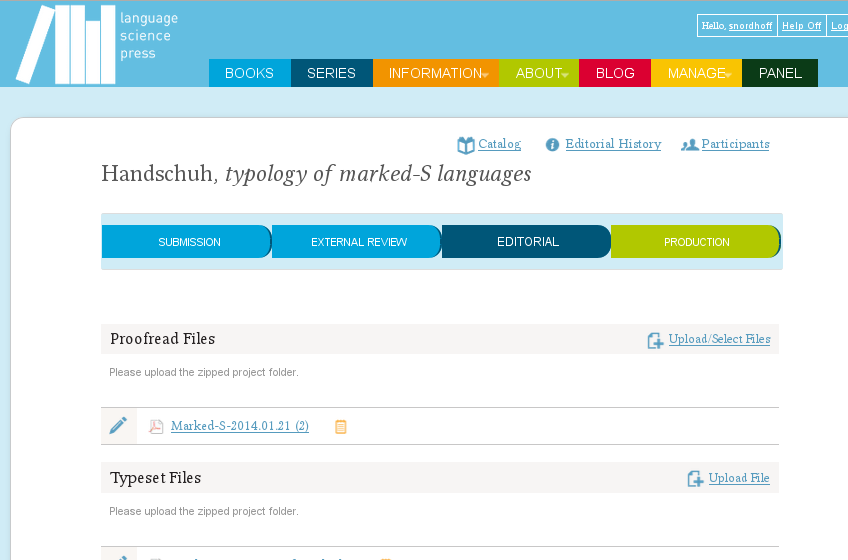
\includegraphics[\width=\textwidth]{./pics/omphandschuh.png}
}



\frame{ 
\frametitle{Was leistet OMP}
\begin{itemize}
 \item   Veröffentlichung
 \item   Metadaten
 \item   Verbreitung (OAI-PMH, Onyx, )
 \item   Datenbankschnittstelle 
\end{itemize}
}

\frame{ 
\frametitle{Was leistet OMP}
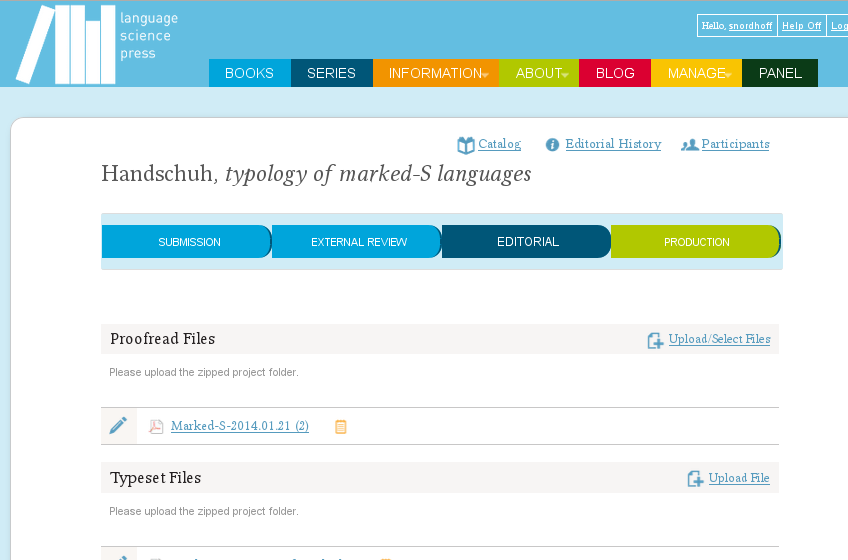
\includegraphics[\width=\textwidth]{./pics/omphandschuh.png}
}

 

\section{Grenzen von OMP}
 

\frame{ 
\frametitle{Grenzen von OMP}
\begin{itemize}
 \item    von Programmierern entwickelt
 \item    Benutzerfreundlichkeit ausbaufähig
 \item    allgemein dürftige Dokumentation 
 \item    ohne Programmierkenntnisse nicht wirklich anpassbar 
\end{itemize}
}

\frame{ 
\frametitle{Grenzen von OMP}
\begin{itemize}
 \item    Rollensystem unklar 
 \item    Stakeholderoverkill
 \item    ISBN, DOI 
 \item    Sammelbände (mehrere Autoren, DOIs pro Beitrag)
\end{itemize}
}

\frame{ 
\frametitle{Grenzen von OMP}
\begin{itemize}
 \item   Keine echte Versionierung
 \item   diverse Bugs
 \item   Blog extern
\end{itemize}
}

 


\section{Weiterentwicklung von OMP}



\frame{
\frametitle{Frametitle1}
  \begin{itemize}
    \item  Höchstwahrscheinlich Orientierung an OJS 
    \item  Einbindung von Weiterentwicklungen Dritter
  \end{itemize}
} 
  

%\setcounter{framenumber}{\thelastpagemainpart}
\end{document}